\setcounter{page}{1}
\section*{Zielsetzung}
In diesem Versuch soll der Grundlagen der Rastertunnelmikroskopie
erlernt werden. Hierzu werden die Oberfläche einer HOPG- (Graphit) und
Goldprobe untersucht. Mit Hilfe der Oberflächenmessung werden die Gittervektoren
der HOPG Struktur bestimmt und ein Höhenprofil des Goldes vermessen.

\section{Theorie}
Die Funktnsweise eines  Rastertunnelmikroskops (RTM) beruht auf den aus der Quantenmechnaik bekannten
\emph{Tunneleffekt}. Dieser erlaubt es Elektron in klassisch verbotene Bereich zu \emph{tunneln}.
Beim Tunneln durchqueren die Elektron ein Potential, welches sie im klassichen Sinne
eigentlich nicht überwinden können (vgl. Abb. \ref{fig: tunneleffekt}).
\begin{figure}[h]
  \centering
  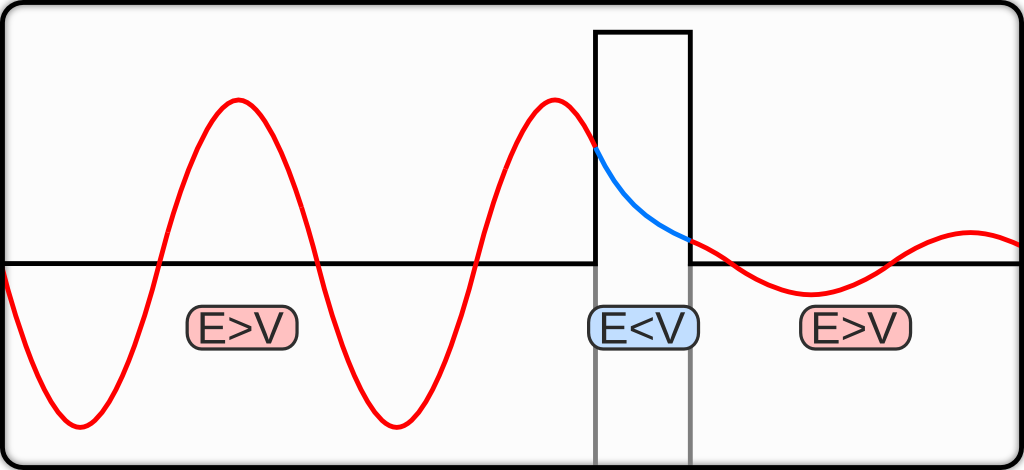
\includegraphics[width=0.6\textwidth]{./pics/tunelleffekt.png}
  \caption{Darstellung des Tunneleffekts \cite{tunnel}.}
  \label{fig: tunneleffekt}
\end{figure}
Zum Beispiel Tunneln die \textbf{Heliumkerne} beim $\alpha$-Zerfall durch das Coulombpotential.

Ein RTM verwendet den Tunneleffekt, um einen \emph{Tunnelstrom} zu erzeugen. Dieser Tunnelstrom
fließt zwischen der Messpitze des Mikroskopen und der Probe. Hierbei ist das zu durch tunnelde
Potential die Luft. Hierbei wird angenommen das sich kein Luftmolekül im Tunnelbereich befindet, welches
die Tunnelwahrscheinlichkeit verringert. Der gemessene Tunnelstrom ist proptional zu

\begin{equation}
  \label{eq: tunnelstrom}
I\propto \frac{U}{d}\exp{-kd\sqrt{\phi}}.
\end{equation}
Dabei ist $d$ der Abstand zwischen Spitze und Probe, $U$ die \textbf{an der Probe anliegende Spannung},
$\phi$ die durchschnittliche Elektronaustrittsarbeit und $k$ eine Konstante die im Vaakum gegeben ist als
\begin{equation*}
  k=\SI{1.025e10}{\per\sqrt{\eV}} \AA.
\end{equation*}

Der Tunnelstrom ist ein Maß für die Elektrondichte und kann verwendet werden um die Oberflächenstruktur
zu rekonstruieren.

\subsection{Piezokeramiken}
Damit Rastertunnelmikroskop Strukturen im Nanometerbeich untersuchen kann, muss
die Spitze sehr genau manövriert werden. Mit Hilfe von Piezokeramiken bzw.
Piezokristallen (vgl. Abb. \ref{}) ist es möglich solche Genauigkeiten zuereichen.
\begin{figure}[h]
  \centering
  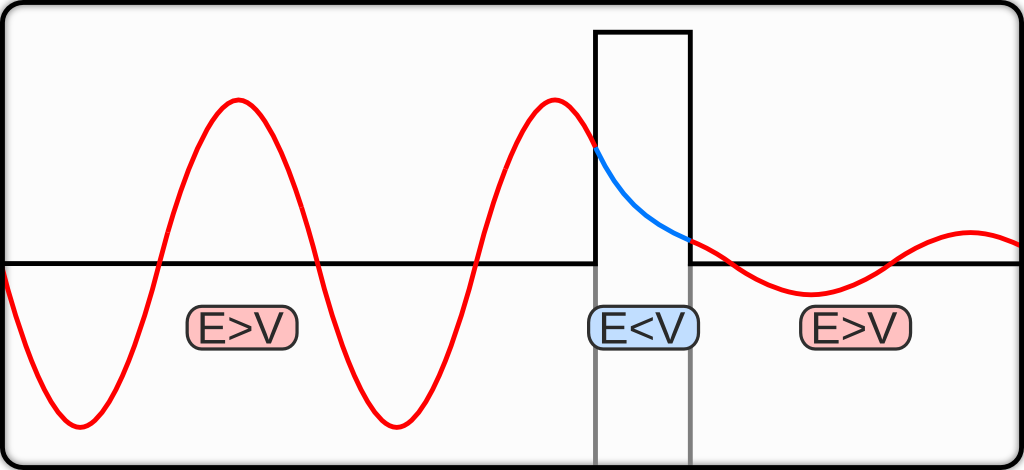
\includegraphics[wi
  ++dth=0.6\textwidth]{./pics/tunelleffekt.png}
  \caption{Darstellung des Tunneleffekts \cite{tunnel}.}
  \label{fig: tunneleffekt}
\end{figure}
Ein Piezokrisall besitzt die Eigenschaft, sich unter Einwirkung eines äußeren
elektrischen Feldes auszudehnen. Dabei findet die Ausdehnung immer parallel zur
Ausrichtung des elektrischen Feldes statt und ist mit den in den Kristall wirkenden
Dipolmomenten zu erklären. In erster Näherung ist die Ausdehnung linear mit der anliegenden Feldstärke,
jedoch ist in Wirklichkeit ein nicht linearer Zusammenhang zwischen Ausdehnung und Feldstärke
gegeben (vgl. Ab.b \ref{fig: non_linear}). Diese Nichtlinearität sorgt dafür das einzelne Bilder des
Rastertunnelmikrsokop nicht einheitlich aussehen.
\begin{figure}[h]
  \centering
  \includegraphics[width=0.6\textwidth]{./pics/nicht_linearität.png}
  \caption{Schematische Darstellung der Nichtlineraität der Auslenkung eines Piezokristalls \cite{rtm}.}
  \label{fig: non_linear}
\end{figure}
Neben der Nichtlineratiät verschlechtern noch weitere
Effekte die Genauigkeit eines RTM. Hierzu gehört zum Beispiel Hystereseeffekte (vgl. Abb. \ref{fig: hysterese}) die dafür sorgen,
das Messungen Richtungsabhängig sind.
\begin{figure}[h]
  \centering
  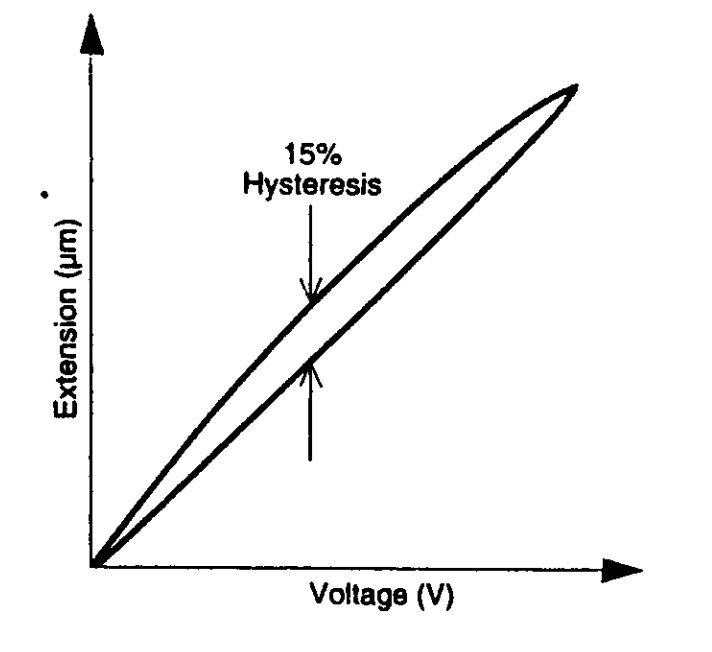
\includegraphics[width=0.6\textwidth]{./pics/hysterese.png}
  \caption{Schematische Darstellung der Hysterese einer Piezokeramik \cite{rtm}.}
  \label{fig: hysterese}
\end{figure}

Bei einer aprupten Spannungsänderung ändert der Kristall seine Auslenkung nicht instantan, sondern benötigt erst eine Gewisse Zeit.
Dieser Effekt, der als \emph{Schleichen} bezeichnet wird, kann bis zu $\SI{100}{\second}$ andauern.
Durch das Schleichen können eigentlich eckige Strukturen gekrümmt aussehen (vgl. Abb. \ref{fig: creep}).
\begin{figure}[h]
  \centering
  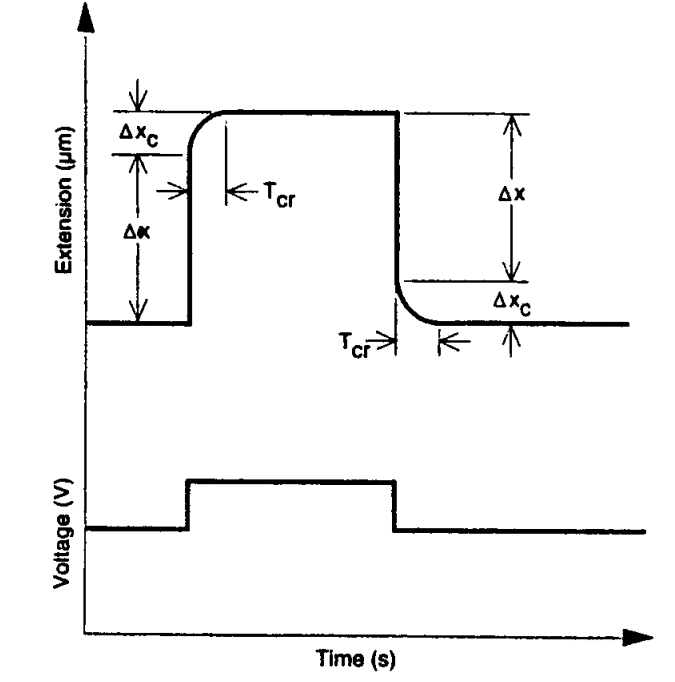
\includegraphics[width=0.6\textwidth]{./pics/creep.png}
  \caption{Auswirkung von Creeps auf eine Messung mit einem RTM \cite{rtm}.}
  \label{fig: creep}
\end{figure}
Außerdem unterliegt ein Piezokeramik einem Effekt der als \emph{Alterung} bezeichnet wird, dieser besagt
das bei langer nicht Verwendung des Kristalls die Ausdehnungsfähigkeit verringert. erklärbar ist der Effekt mit den
Dipolmomenten im Kristalle, die Momente richten sich bei langer nicht Benutzung wirklich aus und verringern
somit die Empfindlichkeit auf äußere Spannungsänderungen (vgl. Abb. \ref{fig: ageing}).
\begin{figure}[h]
  \centering
  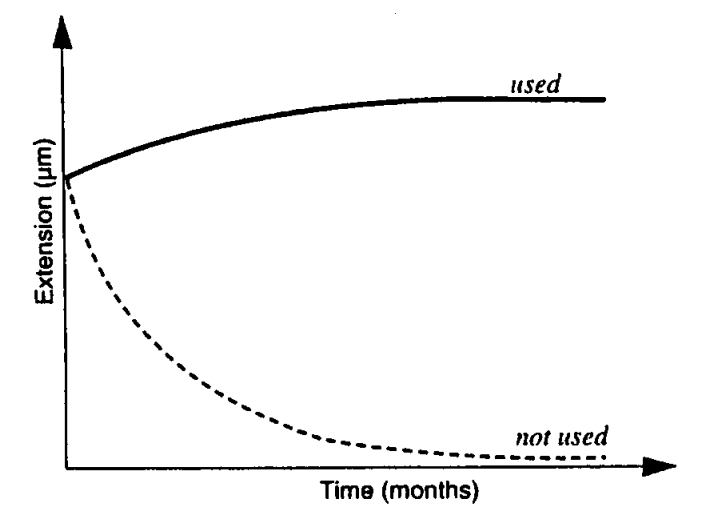
\includegraphics[width=0.6\textwidth]{./pics/ageing.png}
  \caption{Schmeatische Darstelung des Verhalten eines Piezokristall bei häugiger und weniger Benutzung \cite{rtm}.}
  \label{fig: ageing}
\end{figure}
Es ist möglich nach einer Zeit der Nichtverwendung
durch häufiges benutzen die anfängliche Empfindlichkeit wieder zu erlangen.
Das Phänomen der \emph{Kreuzkopplung} beschreibt die $x$- und $y$-Abhängigkeit der $z$-Komponente des Piezokristall (vgl. Abb. \ref{fig: cross_copeling}).
\begin{figure}[h]
  \centering
  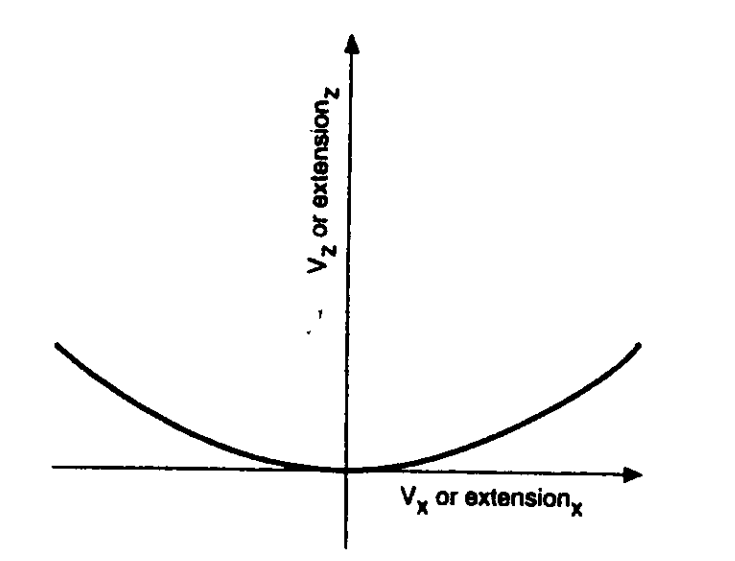
\includegraphics[width=0.6\textwidth]{./pics/cross_copling.png}
  \caption{Schmeatische Darstelung der Auslenkung der Kreuzkopplung \cite{rtm}.}
  \label{fig: cross_copeling}
\end{figure}
Die damit verbundenen Fehlern können mit Hilfe einer Software rausgerechnet werden.

\subsection{HOPG}

\subsection{Gold}
